\chapter{מהטלגרף לסמארטפון}

\begin{epigraph}{}
כל דור בטוח שהוא הראשון שהטכנולוגיה מבלבלת. כל דור טועה, וכל דור צודק.
\end{epigraph}

\section{הודעה שנעה במהירות של רגליים}

במשך רוב ההיסטוריה האנושית, מהירות המידע הייתה שווה למהירות הגוף. ציידת-לקטת שרצתה לספר לשבט השכן שנמצא מעיין חדש הייתה צריכה ללכת לשם. מלך שרצה לשלוח פקודה לגבול הממלכה שלח רץ, ואחר כך פרש. גם האימפריות הגדולות של העולם העתיק, עם הדרכים הסלולות ותחנות הדואר שלהן, לא הצליחו לשבור את החוק הבסיסי הזה: הודעה לא יכולה לנוע מהר יותר מהשליח שנושא אותה.

הדפוס של המאה ה-15 שינה את \textbf{כמות} המידע, אבל לא את מהירותו. ספר מודפס עדיין נסע בעגלה. הידיעה על מותו של מלך יכלה להגיע לפינות הממלכה שבועות אחרי שהוכתר יורשו.

ואז, במאה ה-19, קרה משהו מוזר. המידע התנתק מהחומר.

\section{המברק: כשהמילים עזבו את הסוס}

ב-24 במאי 1844 שלח סמואל מורס את המברק הציבורי הראשון, מוושינגטון לבולטימור. ארבע מילים מהתנ"ך, \en{"What hath God wrought"}, עברו בין שתי הערים כמעט ברגע. לראשונה בהיסטוריה, הודעה הגיעה לפני השליח. למעשה, לא היה שליח בכלל.

קל לזלזל בזה היום, כשהודעת \en{WhatsApp} מגיעה לאוסטרליה בפחות משנייה. אבל עבור בני הדור ההוא זה היה דבר מדהים. עיתונים התחילו לפרסם חדשות מערים רחוקות מאתמול, ולא מהחודש שעבר. בורסות בערים שונות התחילו לנשום באותו קצב. והפילוסופים של התקופה כבר דאגו: האם האנושות מסוגלת לעכל כל כך הרבה מידע, כל כך מהר?

שימו לב לשאלה הזאת. היא תחזור בכל פרק בספר.

\section{מרשת צבאית לרשת עולמית}

בעשורים שאחרי המברק הגיעו הטלפון, הרדיו והטלוויזיה. כל אחד מהם הוסיף משהו: את הקול, את ההמונים, את התמונה. אבל כולם עבדו לפי אותו היגיון: ערוץ אחד, מסר אחד, וקהל שמקבל.

השינוי האמיתי התחיל במעבדות. בסוף אוקטובר 1969 נשלחה ההודעה הראשונה ברשת \en{ARPANET}, מאוניברסיטת \en{UCLA} אל מחשב מרוחק. זו הייתה רשת של חוקרים ושל משרד ההגנה האמריקאי, לא של אזרחים. כמעט אף אחד לא שם לב.

ב-1989 הגיש טים ברנרס-לי, מהנדס תוכנה במעבדת \en{CERN}, מסמך פנימי בשם "ניהול מידע: הצעה" \parencite{berners1989}. הבוס שלו רשם עליו, לפי המסורת, שההצעה "מעורפלת, אבל מרגשת". מן ההצעה המעורפלת הזאת נולד ה-\en{World Wide Web}. האינטרנט הפסיק להיות רשת של מומחים והתחיל להפוך לעיר שבה כולם יכולים לגור.

\begin{thinkbox}
המברק, הטלפון והאינטרנט נולדו כולם מתוך צורך מעשי: עסקים, צבא, מדע. אף אחד מהממציאים לא תכנן לשנות את הדרך שבה מתבגרים מתאהבים או מתווכחים. האם ייתכן שההשפעות החשובות ביותר של טכנולוגיה הן תמיד אלה שאיש לא תכנן?
\end{thinkbox}

\section{המכשיר שבלע את העולם}

ב-9 בינואר 2007 עלה סטיב ג'ובס לבמה והציג את ה-\en{iPhone}. בהודעה לעיתונות תיארה אותו אפל כשלושה מוצרים במכשיר אחד: טלפון נייד, נגן מוזיקה עם מסך מגע, ומכשיר לתקשורת באינטרנט \parencite{apple2007}. בדיעבד, זו הייתה הערכה צנועה מאוד. הסמארטפון בלע גם את המצלמה, המפה, השעון, הפנס, הארנק, הספרייה והטלוויזיה. הוא הפך לשלט הרחוק של החיים כולם.

ואז הגיעו הרשתות החברתיות, שצמחו בשנות ה-2000 וה-2010, והפכו את המכשיר מכלי לקבלת מידע לבמה שעליה כל אחד משדר. ולבסוף, ב-30 בנובמבר 2022, השיקה \en{OpenAI} את \en{ChatGPT} כ"תצוגה מקדימה למחקר" \parencite{openai2022}. לראשונה, המכונה לא רק העבירה את המילים שלנו. היא התחילה לכתוב משלה.

טבלה~\ref{tab:timeline} מסכמת את אבני הדרך העיקריות במסע הזה.

\begin{table}[htbp]
\centering
\caption{ציר זמן: מהמברק לבינה המלאכותית}
\label{tab:timeline}
\begin{tabularx}{\textwidth}{@{}>{\centering\arraybackslash}p{3.9cm} l X@{}}
\toprule
\textbf{שנה} & \textbf{המצאה} & \textbf{מה השתנה} \\
\midrule
1844 & המברק של מורס & המידע נע מהר יותר מהשליח \\
סוף המאה ה-19 & הטלפון & הקול האנושי חוצה מרחקים \\
שנות ה-20 של המאה ה-20 & הרדיו & תקשורת המונים בזמן אמת \\
אמצע המאה ה-20 & הטלוויזיה & התמונה נכנסת לסלון \\
1969 & \en{ARPANET} & מחשבים מתחילים לדבר זה עם זה \\
1973 & הטלפון הנייד & שיחה בלי חוטים, מהרחוב \\
1989 & הצעת ה-\en{Web} ב-\en{CERN} & רשת שכל אחד יכול לגלוש בה \parencite{berners1989} \\
שנות ה-2000 וה-2010 & הרשתות החברתיות & כל אדם הופך לתחנת שידור \\
2007 & ה-\en{iPhone} & האינטרנט עובר לכיס \parencite{apple2007} \\
2022 & \en{ChatGPT} & המכונה מתחילה לכתוב ולשוחח \parencite{openai2022} \\
\bottomrule
\end{tabularx}
\end{table}

\section{כמעט שישה מיליארד}

\begin{sloppypar}
איור~\ref{fig:internet-users} מראה את קצב ההתפשטות. ב-2005 השתמשו באינטרנט כמיליארד בני אדם, כ-15.7\% מאוכלוסיית העולם. ב-2015 היו אלה כ-2.96 מיליארד, וב-2024 כבר כ-5.87 מיליארד, כ-72.3\% מהאנושות \parencite{itu2026data}. בתוך פחות מעשרים שנה, מספר המחוברים גדל כמעט פי שישה.
\end{sloppypar}

% גרף Python: python/make_graphs.py → images/internet_users.png
\begin{figure}[htbp]
\centering
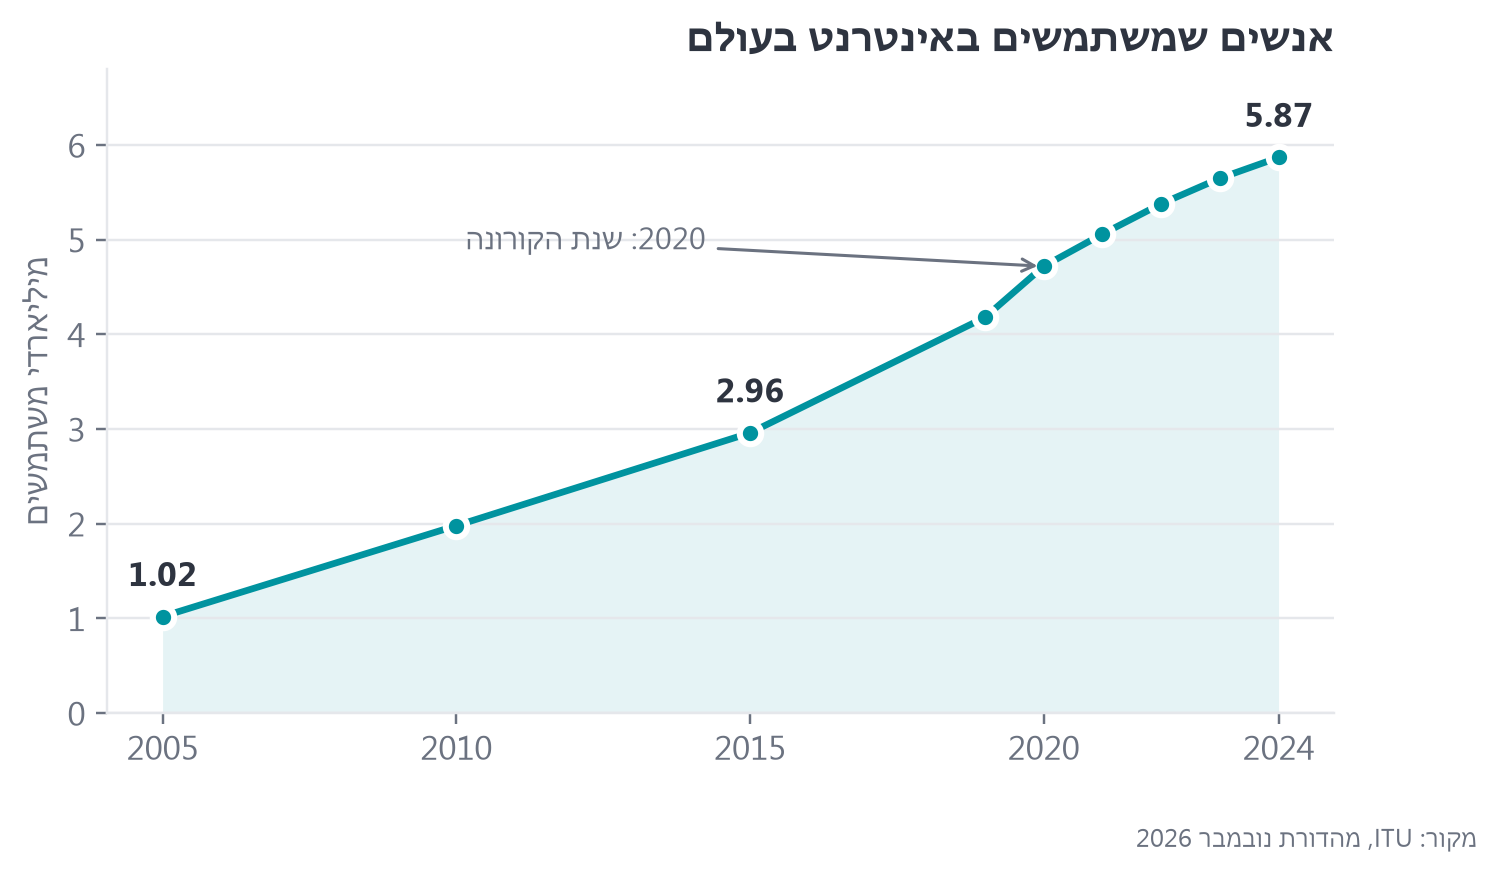
\includegraphics[width=0.92\textwidth]{images/internet_users.png}
\caption{מספר משתמשי האינטרנט בעולם, במיליארדים, 2005--2024 \parencite{itu2026data}. הגרף נוצר ב-\en{Python}.}
\label{fig:internet-users}
\end{figure}


שימו לב לקפיצה שבין 2019 ל-2020: מ-4.18 ל-4.72 מיליארד \parencite{itu2026data}. הנתונים עצמם אינם אומרים מה גרם לקפיצה. ההסבר שמתבקש, וזו פרשנות שלנו ולא ממצא של המקור, הוא מגפת הקורונה, שדחפה אנשים רבים אל המסך, ללימודים, לעבודה ולשיחות עם סבתא. אם זה אכן ההסבר, משבר עולמי אחד עשה בשנה מה שבדרך כלל לוקח כמה שנים.

\begin{factbox}[מספרים שזזים]
גם המספרים עצמם אינם יציבים. במהדורת 2024 של \en{Facts and Figures} העריך איגוד התקשורת הבין-לאומי שבשנה זו היו מחוברים כ-5.5 מיליארד בני אדם \parencite{itu2024}, ואילו בסדרה המעודכנת ההערכה לאותה שנה היא כ-5.87 מיליארד \parencite{itu2026data}. ההבדל נובע מתיקוני מתודולוגיה. בספר הזה אנחנו משתמשים בסדרה המעודכנת בלבד, כדי שהגרף והטקסט ידברו באותה שפה.
\end{factbox}

מהסוס ועד הסמארטפון עברו פחות מ-200 שנה. זה הרף עין במונחים של ההיסטוריה האנושית. הגוף שלנו, המוח שלנו והרגלי השינה שלנו עוצבו במשך מאות אלפי שנים בעולם שבו המידע הגיע לאט. עכשיו הוא מגיע בלי הפסקה. בפרק הבא ננסה להבין מה זה עושה ליום אחד בחיים שלנו.
